\newpage
\renewcommand{\arraystretch}{1.4}
%\section*{Sunday Schedule}
\label{sunday}
\pagestyle{sunday-table}
\setPageBackground
\noindent\begin{landscape}
  \begin{center}
    \enlargethispage{1\baselineskip}
    \noindent\begin{tabular}{Z{0.75cm}Z{2.18cm};{0.2mm/2mm}Z{2.38cm};{0.2mm/2mm}Z{3.26cm};{0.2mm/2mm}Z{1.7cm};{0.2mm/2mm}}
      \cellcolor{commongray}
      &
      \multicolumn{4}{c}{
        \cellcolor{academic}
        HSW 
      }
      \tabularnewline
      \cellcolor{commongray}
      09:00
      \multiColTalk{4}{Z{9.7cm}}{Bridging the Map? Exploring Interactions between the Academic and Mapping Communities in OSM}{A. Yair Grinberger et\,al.}
      \tabularnewline
      \cellcolor{commongray}
      & \multicolumn{1}{c}{\cellcolor{GHS} GHS}
      & \multicolumn{1}{c}{\cellcolor{HSO} HSO}
      & \multicolumn{1}{c}{\cellcolor{academic} HSW}
      & \multicolumn{1}{c}{\cellcolor{KHS} KHS~\noVideo}
      \tabularnewline
      \cellcolor{commongray}
      09:30
      \talk{Flexible Routing with GraphHopper}{Peter Karich}
      \talk{``Mapathon, mapathon, mapathon!''}{Séverin Menard, Nicolas Chavent}
      \talk{OpenStreetMap as a space~\noVideo}{Dipto Sarkar, So Hoi Kay}
      \longTalk{3}{Scholar Lightning Talks}{}
      \tabularnewline
      \programHRule{4}
      \cellcolor{commongray}
      10:00
      \talk{Imagery Solutions in OSM}{Kevin Bullock}
      \talk{Associations dynamics in French speaking Africa\,\diamondSymbol}{Séverin Menard, Nicolas Chavent}
      \talk{Analysis of OSM data through OSM-Notes user posting}{Toshikazu Seto et\,al.}
      &
      \tabularnewline
      \programHRule{4}
      \cellcolor{commongray}
      10:30
      \talk{Lightning Talks III}{}
      \talk{Tales from the Tasking Manager}{Ramya Ragupathy et\,al.}
      \talk{A novel application of models of species abundance to better understand OSM community structure and interactions}{Peter Mooney}
      &
      \tabularnewline
      \programHRule{5}
    \end{tabular}
  \end{center}
  \newpage

  \begin{center}
    \noindent\begin{tabular}{Z{0.75cm}Z{1.80cm};{0.2mm/2mm}Z{1.80cm};{0.2mm/2mm}Z{2.60cm};{0.2mm/2mm}Z{1.40cm};{0.2mm/2mm}Z{1.60cm};{0.2mm/2mm}}
      \cellcolor{commongray}
      & \multicolumn{1}{c}{\cellcolor{GHS} GHS}
      & \multicolumn{1}{c}{\cellcolor{HSO} HSO}
      & \multicolumn{1}{c}{\cellcolor{academic} HSW}
      & \multicolumn{1}{c}{\cellcolor{KHS} KHS~\noVideo}
      & \multicolumn{1}{c}{\cellcolor{Mathematikon C} Mathem. C~\noVideo}
      \tabularnewline
      \rowcolor{commongray}
      11:00
      & \multicolumn{5}{c}{%
      \parbox[c]{24pt}{%
        
\includegraphics[height=10pt]{cafe}%
      }
      break}
      \tabularnewline
      \cellcolor{commongray}
      11:30
      \talk{Overview of map serving architectures}{Paul Norman}
      \talk{Our Falkirk~-- Mitigating the Impacts of Poverty\,\diamondSymbol}{Alison Moon}
      \talk{Towards Scalable Geospatial Remote Sensing for Efficient OSM Labeling\,~\noVideo}{Rui Zhang et\,al.}
      \longTalk{3}{Bilingual Breakout Session}{}
      \longTalk{2}{\emph{Workshop}\linebreak First steps with OpenStreetMap editors}{Angjelina Dervishaj}
      \tabularnewline
      \programCRule{2-4}
      \cellcolor{commongray}
      12:00
      \talk{Customizing Search for Special-Interest Maps}{Sarah Hoffmann}
      \talk{Metrics to monitor Buildings outbounds\,\diamondSymbol}{Pierre Béland}
      \talk{Estimating latent energy demand of buildings}{Nikola Milojevic-Dupont et\,al.}
      &
      &
      \tabularnewline
      \programCRule{2-4}
      \programCRule{6-6}
      \cellcolor{commongray}
      12:30
      \talk{Is your OSM App spying on you?}{Thomas Skowron}
      \talk{Integrating Quality Assurance Checks into Map Editors\,\diamondSymbol}{David Manzer et\,al.}
      \talk{Client-side route planning: preprocessing the OpenStreetMap road network for Routable Tiles}{Harm Delva et\,al.}
      &
      &
      \tabularnewline
      \programHRule{6}
    \end{tabular}
  \end{center}
  \newpage

  \begin{center}
    \noindent\begin{tabular}{Z{0.75cm}Z{1.80cm};{0.2mm/2mm}Z{1.80cm};{0.2mm/2mm}Z{2.60cm};{0.2mm/2mm}Z{1.40cm};{0.2mm/2mm}Z{1.60cm};{0.2mm/2mm}}
      \cellcolor{commongray}
      & \multicolumn{1}{c}{\cellcolor{GHS} GHS}
      & \multicolumn{1}{c}{\cellcolor{HSO} HSO}
      & \multicolumn{1}{c}{\cellcolor{academic} HSW}
      & \multicolumn{1}{c}{\cellcolor{KHS} KHS~\noVideo}
      & \multicolumn{1}{c}{\cellcolor{Mathematikon C} Mathem. C~\noVideo}
      \tabularnewline
      \rowcolor{commongray}
      13:00
      & \multicolumn{5}{c}{%
      \parbox[c]{24pt}{%
        
\includegraphics[height=10pt]{restaurant}%
      }
      lunch}
      \tabularnewline
      \cellcolor{commongray}
      14:00
      \talk{What's behind JOSM?}{Vincent Privat}
      \talk{Spatial Indexes for OSM in PostGIS}{Felix Kunde}
      \talk{Intrinsic assessment of contribution patterns through Exploratory Spatial Data Analysis}{Marco Minghini et\,al.}
      \longTalk{2}{Diversity and Inclusion in OSM}{Patricia Solis et\,al.}
      \longTalk{2}{\emph{Workshop}\linebreak Using OSMCha to understand bad edits}{Andrey Golovin et\,al.}
      \tabularnewline
      \programCRule{2-4}
      \cellcolor{commongray}
      14:30
      \talk{Mapping solar panels can save megatons of CO2}{Dan Stowell, Jerry Clough}
      \talk{Lightning Talks IV}{}
      \talk{Corporate Editors in the Evolving Landscape of OSM: A Close Investigation of the Impact to the Map \& Community}{Jennings Anderson et\,al.}
      &
      &
      \tabularnewline
      \programHRule{6}
    \end{tabular}
  \end{center}
  \newpage

  \begin{center}
    \noindent\begin{tabular}{Z{0.75cm}Z{1.80cm};{0.2mm/2mm}Z{1.80cm};{0.2mm/2mm}Z{2.60cm};{0.2mm/2mm}Z{1.40cm};{0.2mm/2mm}Z{1.60cm};{0.2mm/2mm}}
      \cellcolor{commongray}
      & \multicolumn{1}{c}{\cellcolor{GHS} GHS}
      & \multicolumn{1}{c}{\cellcolor{HSO} HSO}
      & \multicolumn{1}{c}{\cellcolor{academic} HSW}
      & \multicolumn{1}{c}{\cellcolor{KHS} KHS~\noVideo}
      & \multicolumn{1}{c}{\cellcolor{Mathematikon C} Mathem. C~\noVideo}
      \tabularnewline
      \cellcolor{commongray}
      15:00
      \talk{National Trust~-- Managing a Path inventory in OSM: Towards an Open Paths standard in OSM for the UK}{Huw Davies}
      \longTalk{2}{OSM data processing with PostgreSQL/\allowbreak PostGIS}{Jochen Topf}
      \talk{Exploring the Effects of Pokémon Go Vandalism on OSM}{Levente Juhász et\,al.}
      \longTalk{2}{Nomad Maps, an andean cartographic itinerancy by bike \emph{(video)}}{Alban Vivert}
      \bookableSpace
      \tabularnewline
      \programCRule{2-2}
      \programCRule{4-4}
      \programCRule{6-6}
      \cellcolor{commongray}
      15:30
      \talk{Collaborative mapping of cycling infrastructure for route and thematic maps~\diamondSymbol}{Carolina Ortega Espinosa}
      &
      \talk{Analysing the spatio-temporal patterns and impacts of large-scale data production events in OSM}{A. Yair Grinberger et\,al.}
      &
      \bookableSpace
      \tabularnewline
      \rowcolor{commongray}
      16:00
      & \multicolumn{5}{c}{%
      \parbox[c]{24pt}{%
        
\includegraphics[height=10pt]{cafe}%
      }
      break}
      \tabularnewline
    \end{tabular}
  \end{center}
  \newpage

  \begin{center}
    \noindent\begin{tabular}{Z{0.75cm}Z{2.20cm};{0.2mm/2mm}Z{1.40cm};{0.2mm/2mm}Z{2.60cm};{0.2mm/2mm}Z{1.40cm};{0.2mm/2mm}Z{1.60cm};{0.2mm/2mm}}
      \cellcolor{commongray}
      & \multicolumn{1}{c}{\cellcolor{GHS} GHS}
      & \multicolumn{1}{c}{\cellcolor{HSO} HSO}
      & \multicolumn{1}{c}{\cellcolor{academic} HSW}
      & \multicolumn{1}{c}{\cellcolor{KHS} KHS~\noVideo}
      & \multicolumn{1}{c}{\cellcolor{Mathematikon C} Mathem. C~\noVideo}
      \tabularnewline
      \cellcolor{commongray}
      16:30
      \talk{Notes: Can we do better. Experiences and Ideas from the Frontline}{Chris Fleming}
      \talk{Mapper's privacy}{Roland Olbricht}
      \talk{Development after Displacement: Using OSM data to measure SDG indicators at informal settlements}{Hannah Friedrich et\,al.}
      \talk{Updating our attribution guidelines}{Simon Poole}
      \longTalk{2}{\emph{Workshop}\linebreak JOSM Turn Restriction: Improving Data Quality}{Harry Mahardhika Machmud}
      \tabularnewline
      \programCRule{2-5}
      \cellcolor{commongray}
      17:00
      \talk{Is the OSM data model creaking?}{Martin Lucas-Smith}
      \talk{Teams for OpenStreetMap}{Marc Farra}
      \talk{Analysis of OSM data quality at different stages of a participatory mapping process: Evidence from informal urban settings}{Godwin Yeboah et\,al.}
      \longTalk{2}{Local Chapters Congress}{Joost Schouppe}
      &
      \tabularnewline
      \programCRule{2-4}
      \programCRule{6-6}
      \cellcolor{commongray}
      17:30
      \talk{Broken Promises and Technical Difficulties}{Ilya Zverv}
      \talk{Lightning Talks V}{}
      \talk{Assessing the Completeness of Urban Green Spaces in OSM}{Christina Ludwig et\,al.}
      &
      &
      \tabularnewline
      \programHRule{6}
    \end{tabular}
    \newpage

    \label{poster-event}%
    \setlength{\socialEventBoxWidth}{10.82cm}
    \setlength{\socialEventSectionSep}{\baselineskip}
    \noindent\begin{tabular}{Z{0.75cm}Z{\socialEventBoxWidth};{0.2mm/2mm}}
      \rowcolor{ochsenblutrot}
      \parbox[t]{\linewidth}{%
        \textcolor{white}{18:00}%
      }%
      &
      \multicolumn{1}{C{\socialEventBoxWidth}}{%
        \textcolor{white}{%
          Poster Session at Mathematikon
        }%
      }
      \tabularnewline
      \cellcolor{ochsenblutrot}
      &
      \begin{minipage}[t]{\socialEventBoxWidth}
        \vspace{0.2\baselineskip}
        \noindent\begin{minipage}[c]{0.4\linewidth}
          \RaggedRight
          We invite you to join the poster session with the exhibition
          of posters accepted by the academic programme committee and
          the submissions of the open poster competition.

          Drinks, some food and our special State of the Map 2019 beer will be provided.

          \vspace{\socialEventSectionSep}
          \textbf{Location}\\
          Mathematikon\\
          Klaus-Tschira-Platz\\
          69120 Heidelberg\\
          geo:49.4172,8.6755\\
          entrance from the south, ground floor 
          \justifying
        \end{minipage}
        \hfill
        \noindent\begin{minipage}[c]{0.57\linewidth}
          \begin{center}
            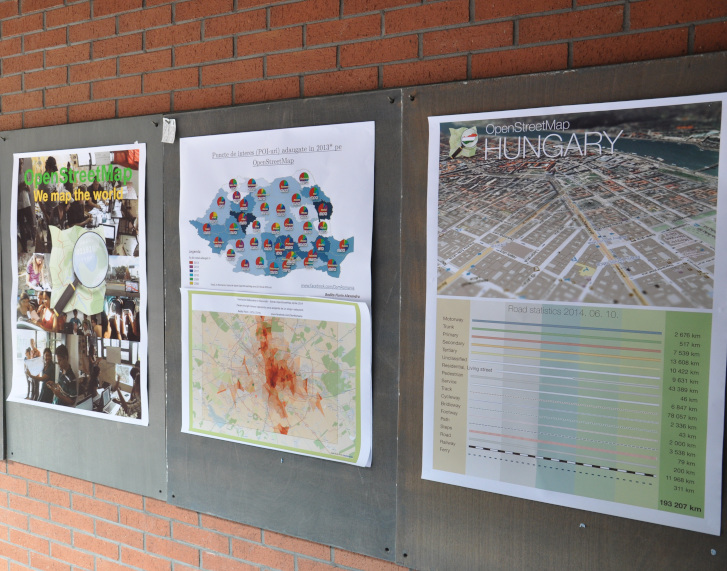
\includegraphics[width=0.9\linewidth]{images-print/posters-sotm-eu-2014.jpg}

            \qrcode[height=18mm,padding]{geo:49.41722,8.67550}%
          \end{center}
        \end{minipage}
      \end{minipage}
      \vspace{0.4\multicolsep}
      \tabularnewline
      \programHRule{2}
    \end{tabular}
  \end{center}
\end{landscape}
\renewcommand{\arraystretch}{1.0}
\normalsize
